\chapter{Preliminary Analysis}\label{Chap:2}

\section{Challenges}

In the attempt to tackle the problem, various challenges arise that are worth mentioning.

\subsection{Feature Selection}\label{SSec: features}

Features are pieces of information that may be useful for predictions. It is generous of Kaggle to provide a comprehensive collection of data. However, not all data is relevant to making predictions. Before a set of features can be selected, careful choices must be made on which data sets to use and which portion of that data set is relevant to solving the problem. 

Regardless of the machine-learning technique used, the most obvious choice of data sets to use is the historical match records for both regular and tournament seasons. However, some data sets contain match records that date back to as early as 1985, which are no longer relevant in today's context. After all, the NCAA tournament teams consist of \emph{college students} who can only stay with a team for a maximum of four years before graduation. As players constantly leave and join the team, it is difficult to quantify the effect brought by changes in a team's composition on the strength of that team, given only the team-level data. Moreover, there were some substantial updates on the Tournament's rules at the beginning of the 2008-2009 season~\cite{NP15}, which also affected the strategies teams used in the subsequent tournaments. Therefore, only the most recent match records are useful for prediction. For the purpose of this project, a four-year window from 2013 to 2016 is selected and all data used in this project fall within this window. In addition, only the match records from the regular seasons are actually used, since there are only a few records from the tournament seasons which add little value to making predictions. 

There are a number of potential features that can be selected from the data set \textbf{RegularSeasonDetailedResult}. The potential features are further categorised as basic and additional features. Table~\ref{Ta:basic_feature} gives a summary of the basic features. 

\begin{table}[h!]
\centering
\begin{tabular}{ | l | l | }
\hline
\textbf{Feature} & \textbf{Description} \\ \hline
Wteam & The id number of the team that won the game \\ \hline
Wscore & The number of points scored by the winning team \\ \hline
Lteam & The id number of the team that lost the game \\ \hline
Lscore & The number of points scored by the losing team \\ \hline
Wloc & The location of the winning team \\ \hline
Numot & The number of overtime periods in the game \\ \hline
\end{tabular}
\caption{A Summary of the Basic Features}\label{Ta:basic_feature}
\end{table}

The additional features describe both \emph{offensive} and \emph{defensive} strengths of both winning team and losing team. Table~\ref{Ta:offensive_feature} gives a summary of features describing offensive strengths, while Table~\ref{Ta:defensive_feature} focuses on defensive strengths. Although the two tables list features from the winning team's perspective, another duplicated set of features also exists for the losing team. 

\begin{table}[h!]
\centering
\begin{tabular}{ | l | l | }
\hline
\textbf{Feature} & \textbf{Description} \\ \hline
Wfgm & The number of field goals made by the winning team\\ \hline
Wfgm3 & The number of three pointers made by the winning team \\ \hline
Wftm & The number of free throws made by the winning team \\ \hline
Wor & The number of offensive rebounds by the winning team \\ \hline
Wto & The number of turnovers by the winning team\\ \hline
Wast & The number of assists by the winning team \\ \hline
Wstl & The number of steals by the winning team \\ \hline
Wblk & The number of blocks by the winning team \\ \hline
\end{tabular}
\caption{A Summary of the Offensive Features}\label{Ta:offensive_feature}
\end{table}

\begin{table}[h!]
\centering
\begin{tabular}{ | l | l | }
\hline
\textbf{Feature} & \textbf{Description} \\ \hline
Wfga & The number of field goals attempted by the winning team \\ \hline
Wfga3 & The number of three pointers attempted by the winning team\\ \hline
Wfta & The number of free throws attempted by the winning team\\ \hline
Wdr & The number of defensive rebounds by the winning team \\ \hline
\end{tabular}
\caption{A Summary of the Defensive Features}\label{Ta:defensive_feature}
\end{table}

The potentially many features make model selection challenging, because they create an exponential number of possible models. If a feature has $m$ possible values, to select the best models based on $n$ features, at least $\Theta(n^{m})$ models have to be examined, which is impractical given that only one submission is allowed at one time. Therefore, this project uses a greedy strategy where all other features are fixed at their optimal values when one feature varies to select a suboptimal model. 

\subsection{Interrelationship}

No team is in isolation. The tournament matches are interactive processes whereby complex interrelationships exist amongst all the contesting teams, which adds another layer of complication in the attempt to predict match results. For example, given the history match records that Team A beaten Team B and Team C lost to Team B, one should intuitively conclude that Team A should have a higher probability of beating Team C. But what if another record shows that Team A once lost to Team C? In that case, the relative strength levels of the three teams will be hard to determine based purely on that intuition. Moreover, the match whose result is to be predicted may be the very \emph{first} match ever between two teams. In other words, there are no historical records that give a direct assessment on the two teams' relative strengths. Such lack of knowledge must be complemented by some forms of inference based on the interrelationships amongst the teams. So a good predictive model should not only be able to take into consideration the current game record, but also explore the interrelationships amongst all the game records and generalise on unseen matches. 

\subsection{The Curse of Model Popularity}
The problem to solve can be categorised as a classification problem under supervised learning. But since the final answers to be submitted are in fact \emph{probabilities}, non-probabilistic models like support vector machines will hardly work. Therefore, the first a few models attempted in this project include the most popular ones: logistic regression and multilayer perceptrons. 

The inputs to these popular models are the seed positions of each team, since the seeds represent an official view on the relative strength of each team. However, the performances of these models are not as good as expected: the logistic model only gives a \nth{283} position on the leaderboard. Moreover, only teams in a tournament are assigned a seed but the number of tournament matches is not large enough to support accurate predictions. Although~\cite{PJ06} suggests a combination of logistic regression and Markov chain to predict match outcomes, these popular models alone based on simply seeds are unlikely to give a good result. 

\section{Approach}\label{Sec: approach}
In light of the challenges identified, the general approach is to quantitatively describe the \emph{skill} of each team, from which the winning probabilities are derived. This section gives a rough idea about the approach used in this project, while the detailed mathematical principles are left to Chapter~\ref{Chap:3}. 

The system used to estimate the skill of a team is known as a \emph{rating system}. An example of a rating system is the famous Elo rating system~\cite{AE78} widely applied in board games like chess and Go. In a Gaussian rating system, each team $i$ is assumed to have a skill $s_{i}$ that follows a Gaussian distribution $s_{i} \sim \mathcal{N}(\mu_{i}, \sigma_{i}^{2})$, where $\mu_{i}$ is the mean skill of a team and $\sigma_{i}$ can be considered as the system's \emph{belief} about the team's skill level. 

Depending on the rating system, the skill of a team is updated after a single match or a series of matches within a specific period. The amount of such a update depends on how \emph{surprising} a match outcome is --- if, prior to a match, Team A is expected to have a very high probability of beating Team B based on their \emph{skill gap}, an outcome that Team A actually wins the game will \emph{not} result in a significant update on either Team A's or Team B's skill; however, on the other hand, if it turns out that Team B performs superbly and beats Team A at the end of the match despite its lower skill level, which is known as an ``upset'' in sport term, there \emph{will} be a significant increase in Team B's skill and a significant decrease in Team A's skill. But in either case, the belief of skills $\sigma_{i}$ will shrink because the rating system becomes more confident about the two teams' skill level. 

As an example, suppose two teams have the same initial skill estimates of $s_{i}$ and $s_{j}$ respectively as shown in Figure~\ref{Fig:t_0}. As the tournament begins, $s_{i}$ and $s_{j}$ are adjusted according to the outcomes of the matches, which is represented by the shift of skill curves as shown in Figure~\ref{Fig:t_1} and~\ref{Fig:t_2}. In the meanwhile, the skill curves become increasingly \emph{taller}, indicating that the rating system is increasingly confident about their skill levels. Finally when the tournament ends, the rating system reports the final standings of the two teams as shown in Figure~\ref{Fig:t_3}.
\begin{figure}[h!]

\begin{subfigure}{.5\textwidth}
\centering
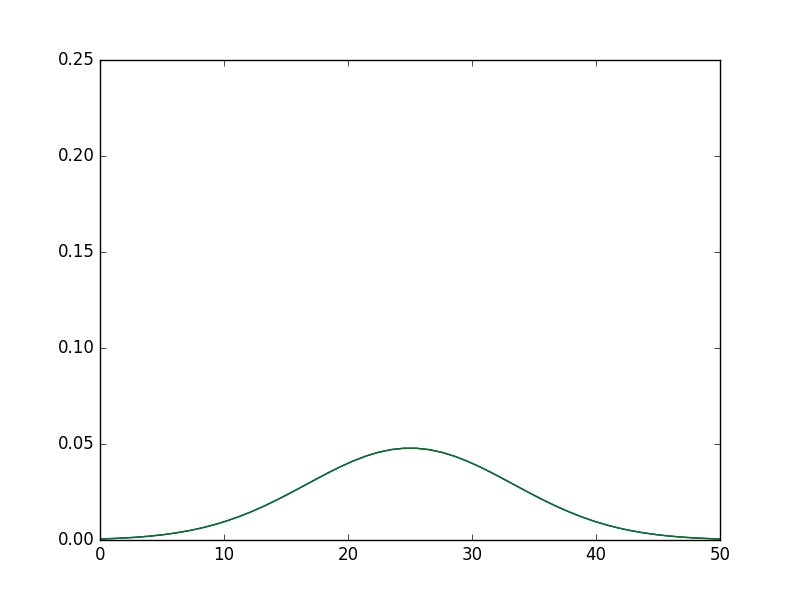
\includegraphics[width = .9\linewidth]{0}
\caption{Timestamp $t = 0$}
\label{Fig:t_0}
\end{subfigure}
\begin{subfigure}{.5\textwidth}
\centering
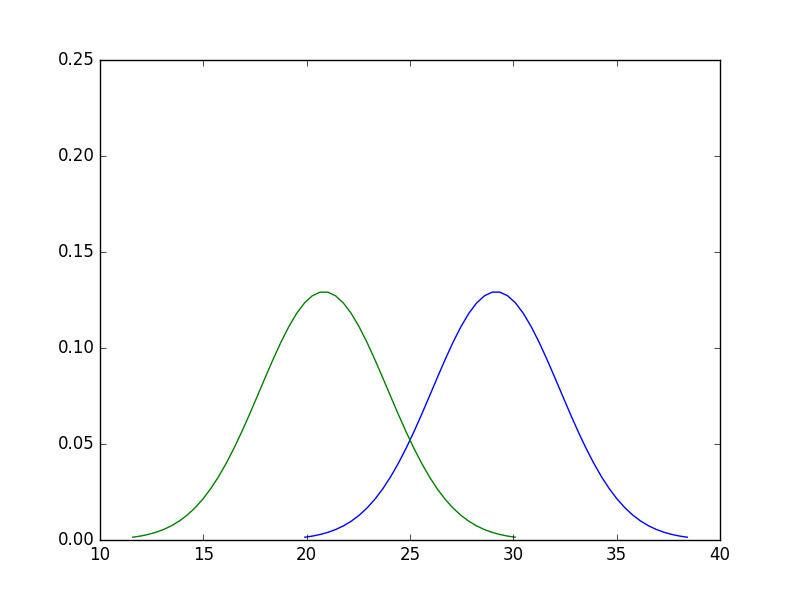
\includegraphics[width = .9\linewidth]{12}
\caption{Timestamp $t = 1$}
\label{Fig:t_1}
\end{subfigure}

\begin{subfigure}{.5\textwidth}
\centering
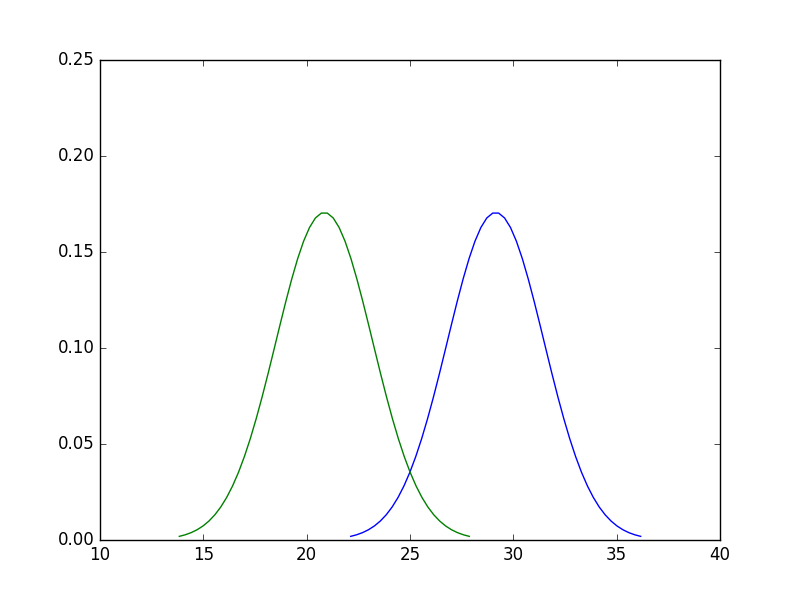
\includegraphics[width = .9\linewidth]{24}
\caption{Timestamp $t = 2$}
\label{Fig:t_2}
\end{subfigure}
\begin{subfigure}{.5\textwidth}
\centering
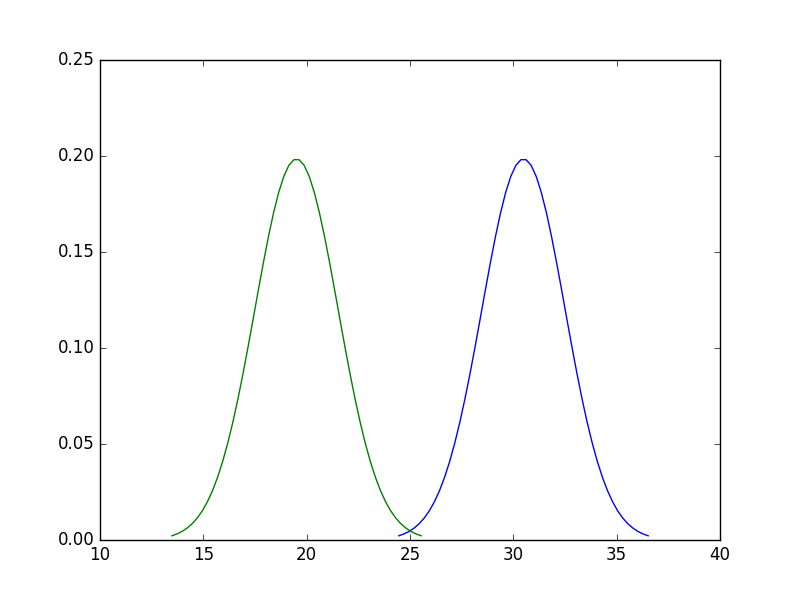
\includegraphics[width = .9\linewidth]{36}
\caption{Timestamp $t = 3$}
\label{Fig:t_3}
\end{subfigure}

\caption{An Example of Skill Update}
\label{Fig:skill_update}
\end{figure}

A team's probability of beating another team in an \emph{upcoming} match can be estimated from the two teams' skill difference. 
\begin{equation}
P(s_{i} > s_{j}) = \Phi(\frac{\mu_{i} - \mu_{j}}{\sqrt{\sigma_{i}^{2} + \sigma_{j}^{2}}})
\end{equation}
where $\Phi$ is the cumulative distribution function of a standard Gaussian distribution.